\chapter{Gesamtsystem}

Das Gesamtsystem besteht softwareseitig aus einer Kombination öffentlich verfügbarer und eigens erstellter \ac{ROS}-Pakete. Das Programm ist so gestaltet, dass die Roboter- und Bilderkennungshardware, wenn passende Konfigurationsdateien für Kamerasystem und Roboterspezifikation vorhanden sind, variabel sind. Folgendes Kapitel bietet einen Überblick über die Aufgaben aller verwendeten Pakete und die Struktur des gesamten Systems mit Fokus auf der Objekterkennung sowie den zeitlichen Ablauf eines einzelnen Bewegungsschrittes.

\textbf{Hinweis}: Das in diesem Kapitel beschriebene Gesamtsystem ist noch nicht vollständig implementiert. Die Ansteuerung des Greifers ist aufgrund von Kommunikationsproblemen mit der verwendeten Reis Robotersteuerung nicht funktionsfähig und muss somit manuell bedient werden. Die Schnittstelle zwischen der Objekterkennung und Handhabung funktioniert aktuell ausschließlich, wenn nur ein einzelner beliebiger Block vom Kamerasystem erkannt wird. Zu Demonstrations- und Testzwecken werden daher zwei Algorithmen zur Verfügung gestellt: für die intelligenten Handhabungssequenzen der Teile wird ein fester Bauplan für Start- und Zielposition vorgegeben\aus.
Zur Nutzung der Bilderkennung in Verbindung mit der Bewegung der Objekte wird der in \refSec{subsec:algorithmus_positionserkennung} beschriebene Algorithmus genutzt.


\section{Programmstruktur} \label{sec:programmstruktur}

Die Zusammenhänge aller Programme sind in \refFig{fig:gesamtsystem_struktur} aufgeführt. Hier wird verstärkt auf die Objekterkennung (rot) eingegangen. Die Roboterbewegung wird in einer Arbeit von Steinbeck \cite[Abschnitt~4.1]{steinbeck_entwicklung_2022} behandelt.

\begin{figure}[ht]
    \centering
    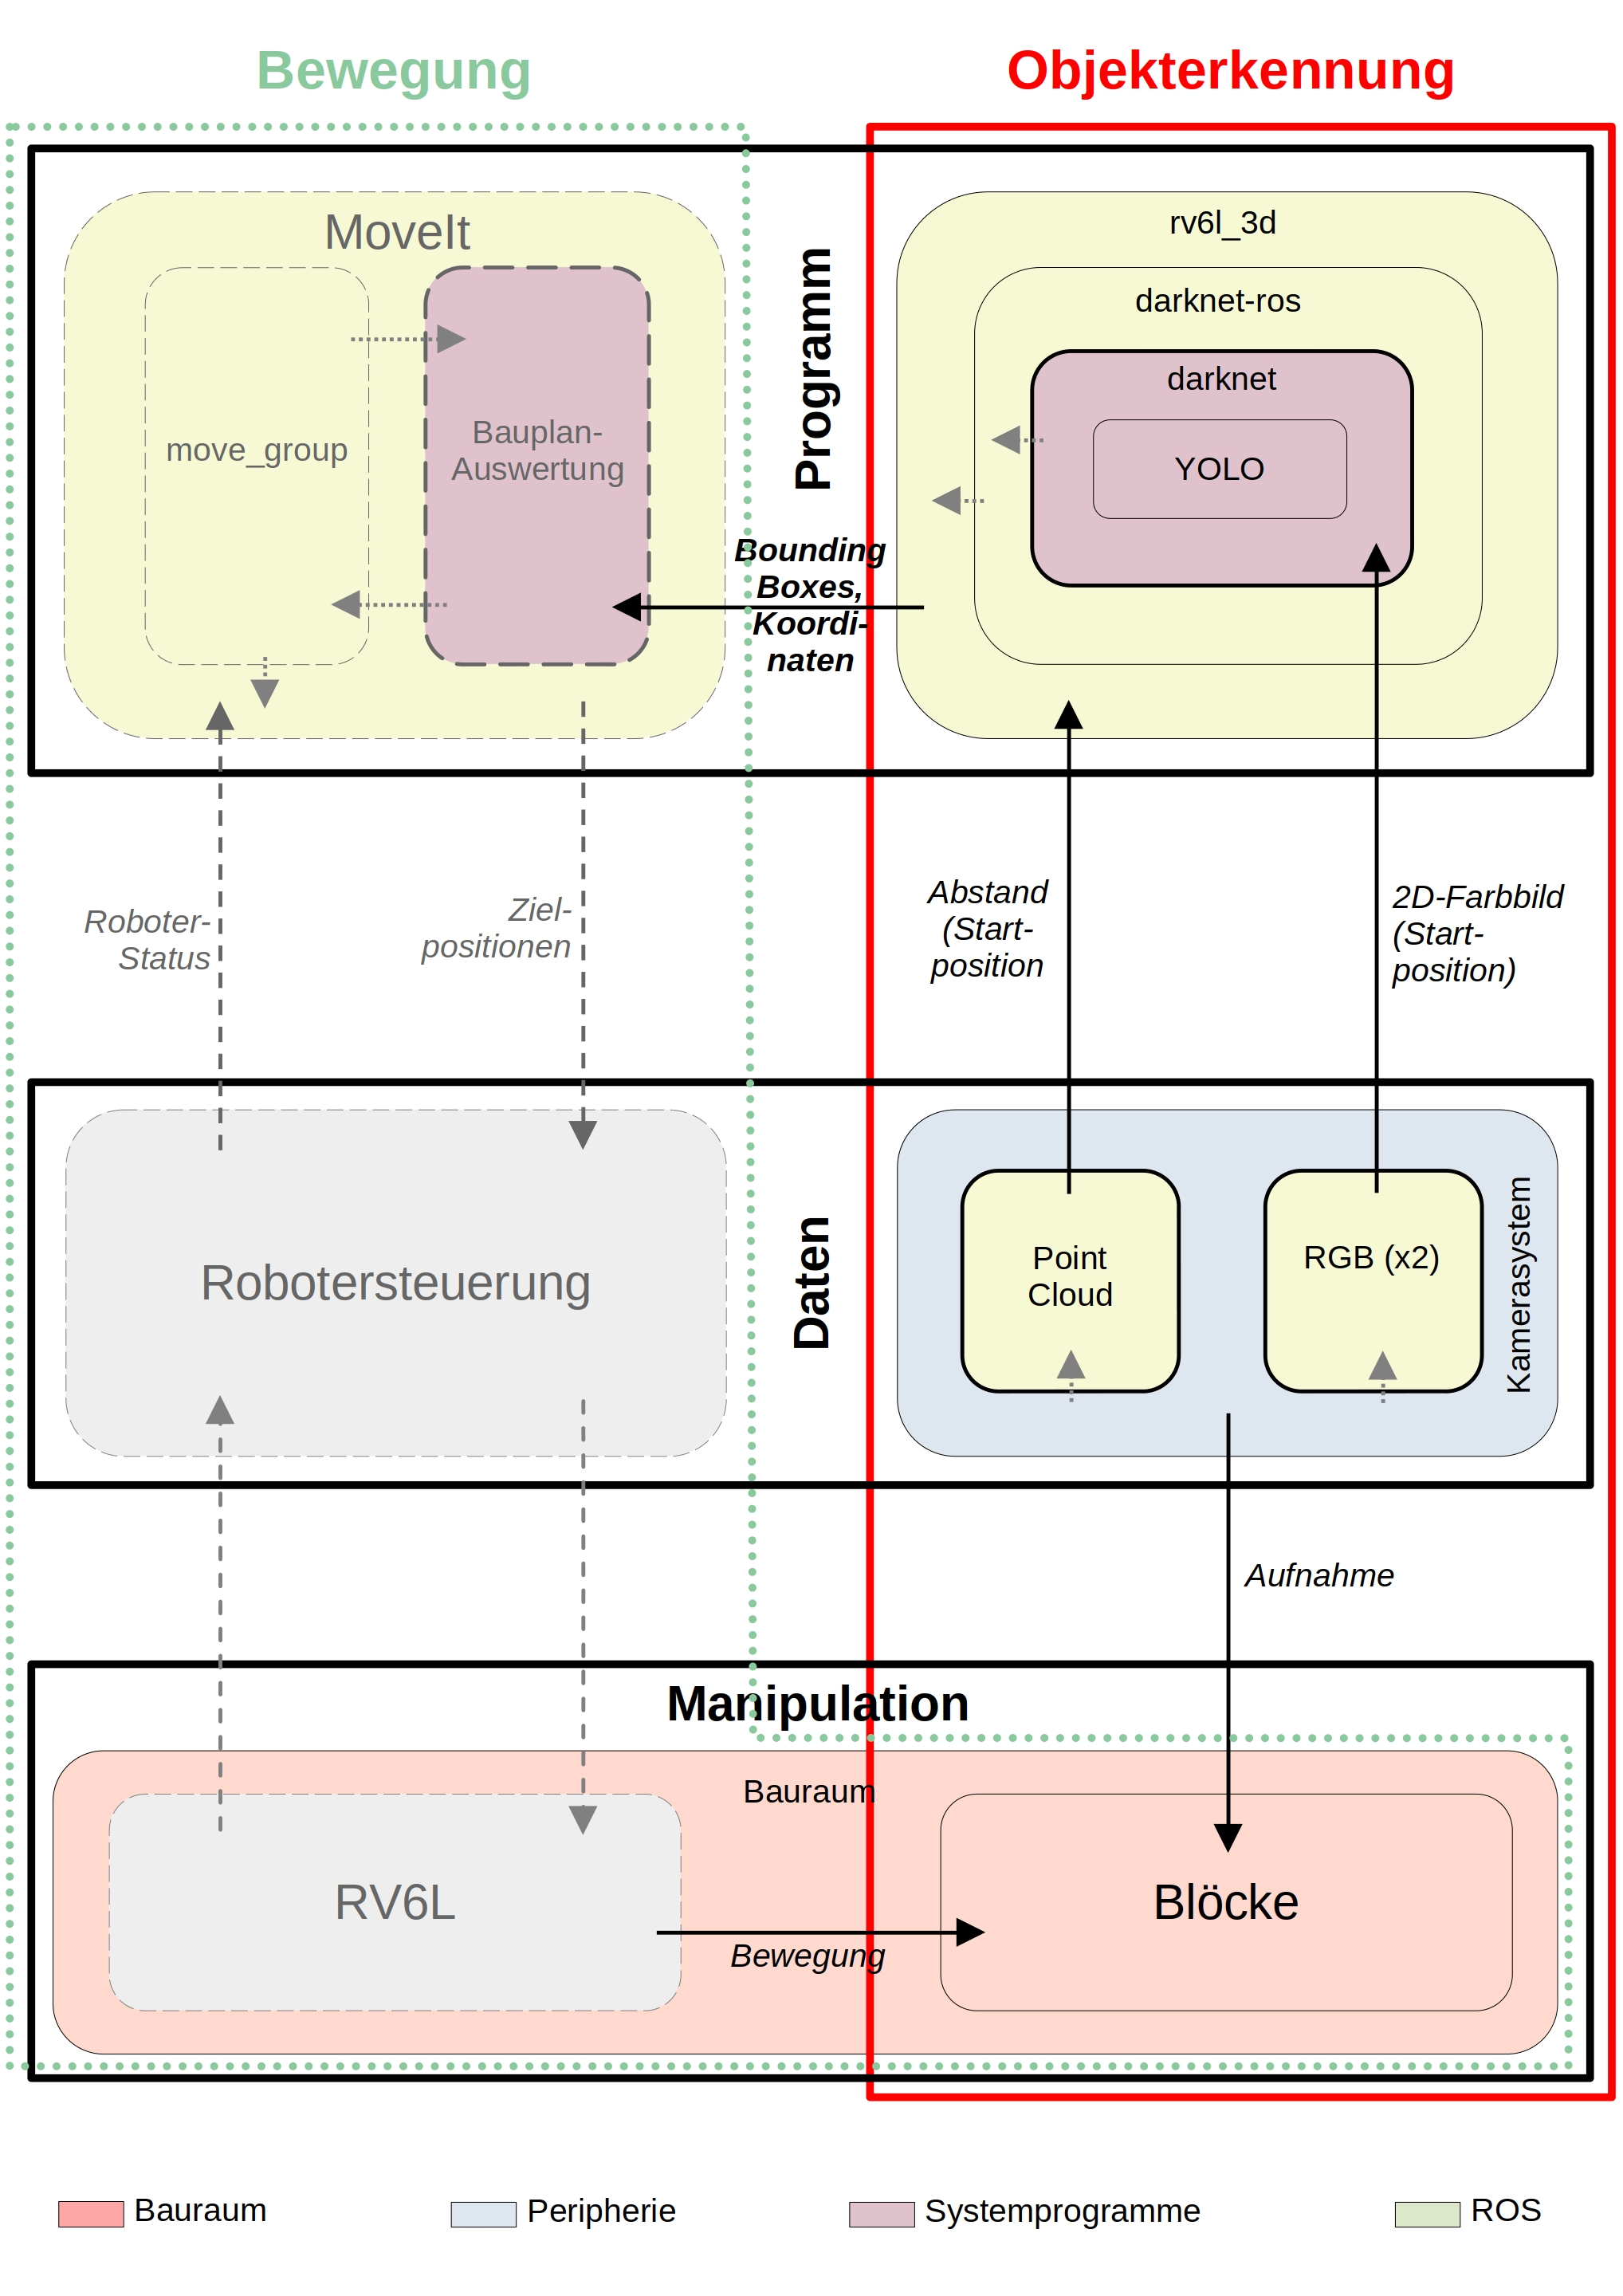
\includegraphics[width=\textwidth]{Bilder/gesamtsystem_struktur.jpg}
    \caption{Struktur des Gesamtsystems}
    \label{fig:gesamtsystem_struktur}
\end{figure}

Die Eingangsdaten des Systems bilden die Daten der beiden RGB-Kameras und der 3D-\textit{Point Cloud}. Diese nimmt mithilfe des RealSense-Treibers für \ac{ROS} ein Bild der Bauteile im Arbeitsbereich auf. Da es sich bei der RealSense um eine Stereokamera handelt, wird aus den Bildern beider Kameras mit Unterstützung der Punkte des Infrarotprojektors eine \textit{Point Cloud} berechnet, die anschließend vom \textit{rv6l\_3d}-Paket verwendet wird. Ein RGB-Bild der Kamera wird außerdem an das \textit{Darknet}-Framework und von dort an \textit{darknet\_ros} weitergegeben.

Die Grundlage der Erkennung bildet der \textit{\ac{YOLO}}-Algorithmus. Dieser wird vom \textit{Darknet}-Framework, was auch zum Training des Algorithmus verwendet wird, zur Erkennung der Objekte genutzt.  Es gibt die Objektklasse und jeweils die Koordinaten des oberen linken und unteren rechten Punktes der \textit{Bounding Boxes} zurück. Diese Koordinaten sind in Pixeln mit dem Mittelpunkt als Ursprung des 2D-Koordinatensystems angegeben. Für die Interaktion mit \ac{ROS} ist das Paket \textit{darknet\_ros} zuständig. Dieses nutzt einen \textit{Subscriber} zur Verwendung von Kameradaten und -aufnahmen und gibt relevante Daten an \textit{Darknet} weiter. Daraufhin extrahiert es relevante Informationen, die von \textit{Darknet} zurückgegeben werden. Unter Nutzung dieser Daten erfolgt eine Bereitstellung eigener \textit{Topics}, beispielsweise mit den Koordinaten der \textit{Bounding Boxes}, einer Visualisierung dieser und den Objektklassen.

Da die Position in Pixeln mit dem Abstand der Objekte variiert, werden für die Handhabung der Bauteile aufgrund der variablen Höhe und der wechselnden Kameraposition \textit{Bounding Box}-Koordinaten in einer abstandsunabhängigen Einheit benötigt. Dafür wird von dem in \refSec{subsec:rv6l_3d} erwähnten \textit{rv6l\_3d}-Paket unter Nutzung von Abstands- und Hardwareinformationen der 3D-Kamera und den \textit{Bounding Box}-Koordinaten eine Position in Metern relativ zum Kameramittelpunkt berechnet. Durch die Anpassung des Pakets auf den vorliegenden Anwendungsfall erfolgt keine Rückgabe der gesamten \textit{Bounding Box}, sondern der dreidimensionalen Position des Mittelpunktes der Objektoberfläche relativ zum Ursprung des Kamerakoordinatensystems. Dazu werden die Informationen aus dem \textit{darknet\_ros}-Paket mit den \textit{Point Cloud}-Daten des verwendeten Kamerasystems abgeglichen.

\section{Programmablauf}
Dieser Abschnitt beschreibt die Abläufe beim Start des Gesamtprogramms.

\begin{description}
    \item[1: Hardware-Interface] Zuerst werden die Programme für die Kommunikation zwischen \ac{ROS} und der Robotersteuerung und für die Interaktion mit dem realen Roboter gestartet.
    \item[2: Bilderkennung] Der für die Objektklassifikation und Positionserkennung zuständige \textit{Node} wird gestartet
    \item[3: Bewegungsalgorithmus] Zuletzt wird der Bewegungsalgorithmus gestartet. Dieser nutzt die Daten der Bilderkennung zur Berechnung der Objektpositionen und zum anschließenden Anordnen der Objekte nach dem vorgegebenen Bauplan.
\end{description}

\section{Bewegungsablauf}

\refFig{fig:gesamtsystem_ablauf} zeigt den Ablauf der gesamten Roboterbewegung nach Programmstart. Dieser kann in folgende Schritte unterteilt werden:

\begin{description}
    \item[1: Startposition] \beh Die Startposition kann beliebig gewählt werden, solange es sich nicht um eine singuläre Pose handelt.
    \item[2: Position für die Bilderkennung] Diese Position mit einer Höhe von $0,60m$ über der Tischebene stellt einen Kompromiss zwischen Zuverlässigkeit der Bilderkennung und Abdeckung des Arbeitsraumes, in dem sich die zufällig angeordneten Objekte befinden, dar. Diese Position kann je nach Anwendung individuell gewählt werden und hängt vom verwendeten Algorithmus, dem Datensatz zum Einlernen des Algorithmus, der Auflösung der Kamera und der Anzahl der Objekte ab.
    \item[3: 2D-Lokalisierung] Dieser Schritt ist notwendig, damit das System die Anzahl und Klasse der verwendeten Teile sowie eine ungefähre Position aller Objekte erfassen kann. Der in \refSec{subsec:intel_realsense} erwähnte Distanzbereich ist hier irrelevant, da nur die Position in horizontaler Ebene benötigt wird.
    \item[4: Teilmittelpunktposition] \beh Hier wird mithilfe des in Schritt 3 erkannten Mittelpunktes des ersten Objekts eine genauere Mittelpunktposition ausfindig gemacht.
    \item[5: 3D-Lokalisierung] Für die Lokalisierung wird das in \refSec{subsec:rv6l_3d} beschriebene Paket verwendet. Sobald sich die Kamera näherungsweise über dem Objektmittelpunkt befindet, wird der Abstand zwischen Kamera und dem durch eine \textit{Point Cloud} erkannten höchsten Punkt des Objekts ermittelt. Dieser Punkt wird in Form einer Liste aus vier Variablen mit Relativposition zur Kamera und Objektklasse zurückgegeben.
    \item[6: Zielposition] \beh Die im Bauplan festgelegte Zielposition des Teils wird angefahren.
    \item[7: Endposition] Nach Ablegen aller Teile kann der Roboter in eine beliebige, nicht singuläre Pose fahren.
\end{description}

Die Schritte \textbf{4} bis \textbf{6} werden für jedes Teil wiederholt.

\begin{figure}[ht]
    \centering
    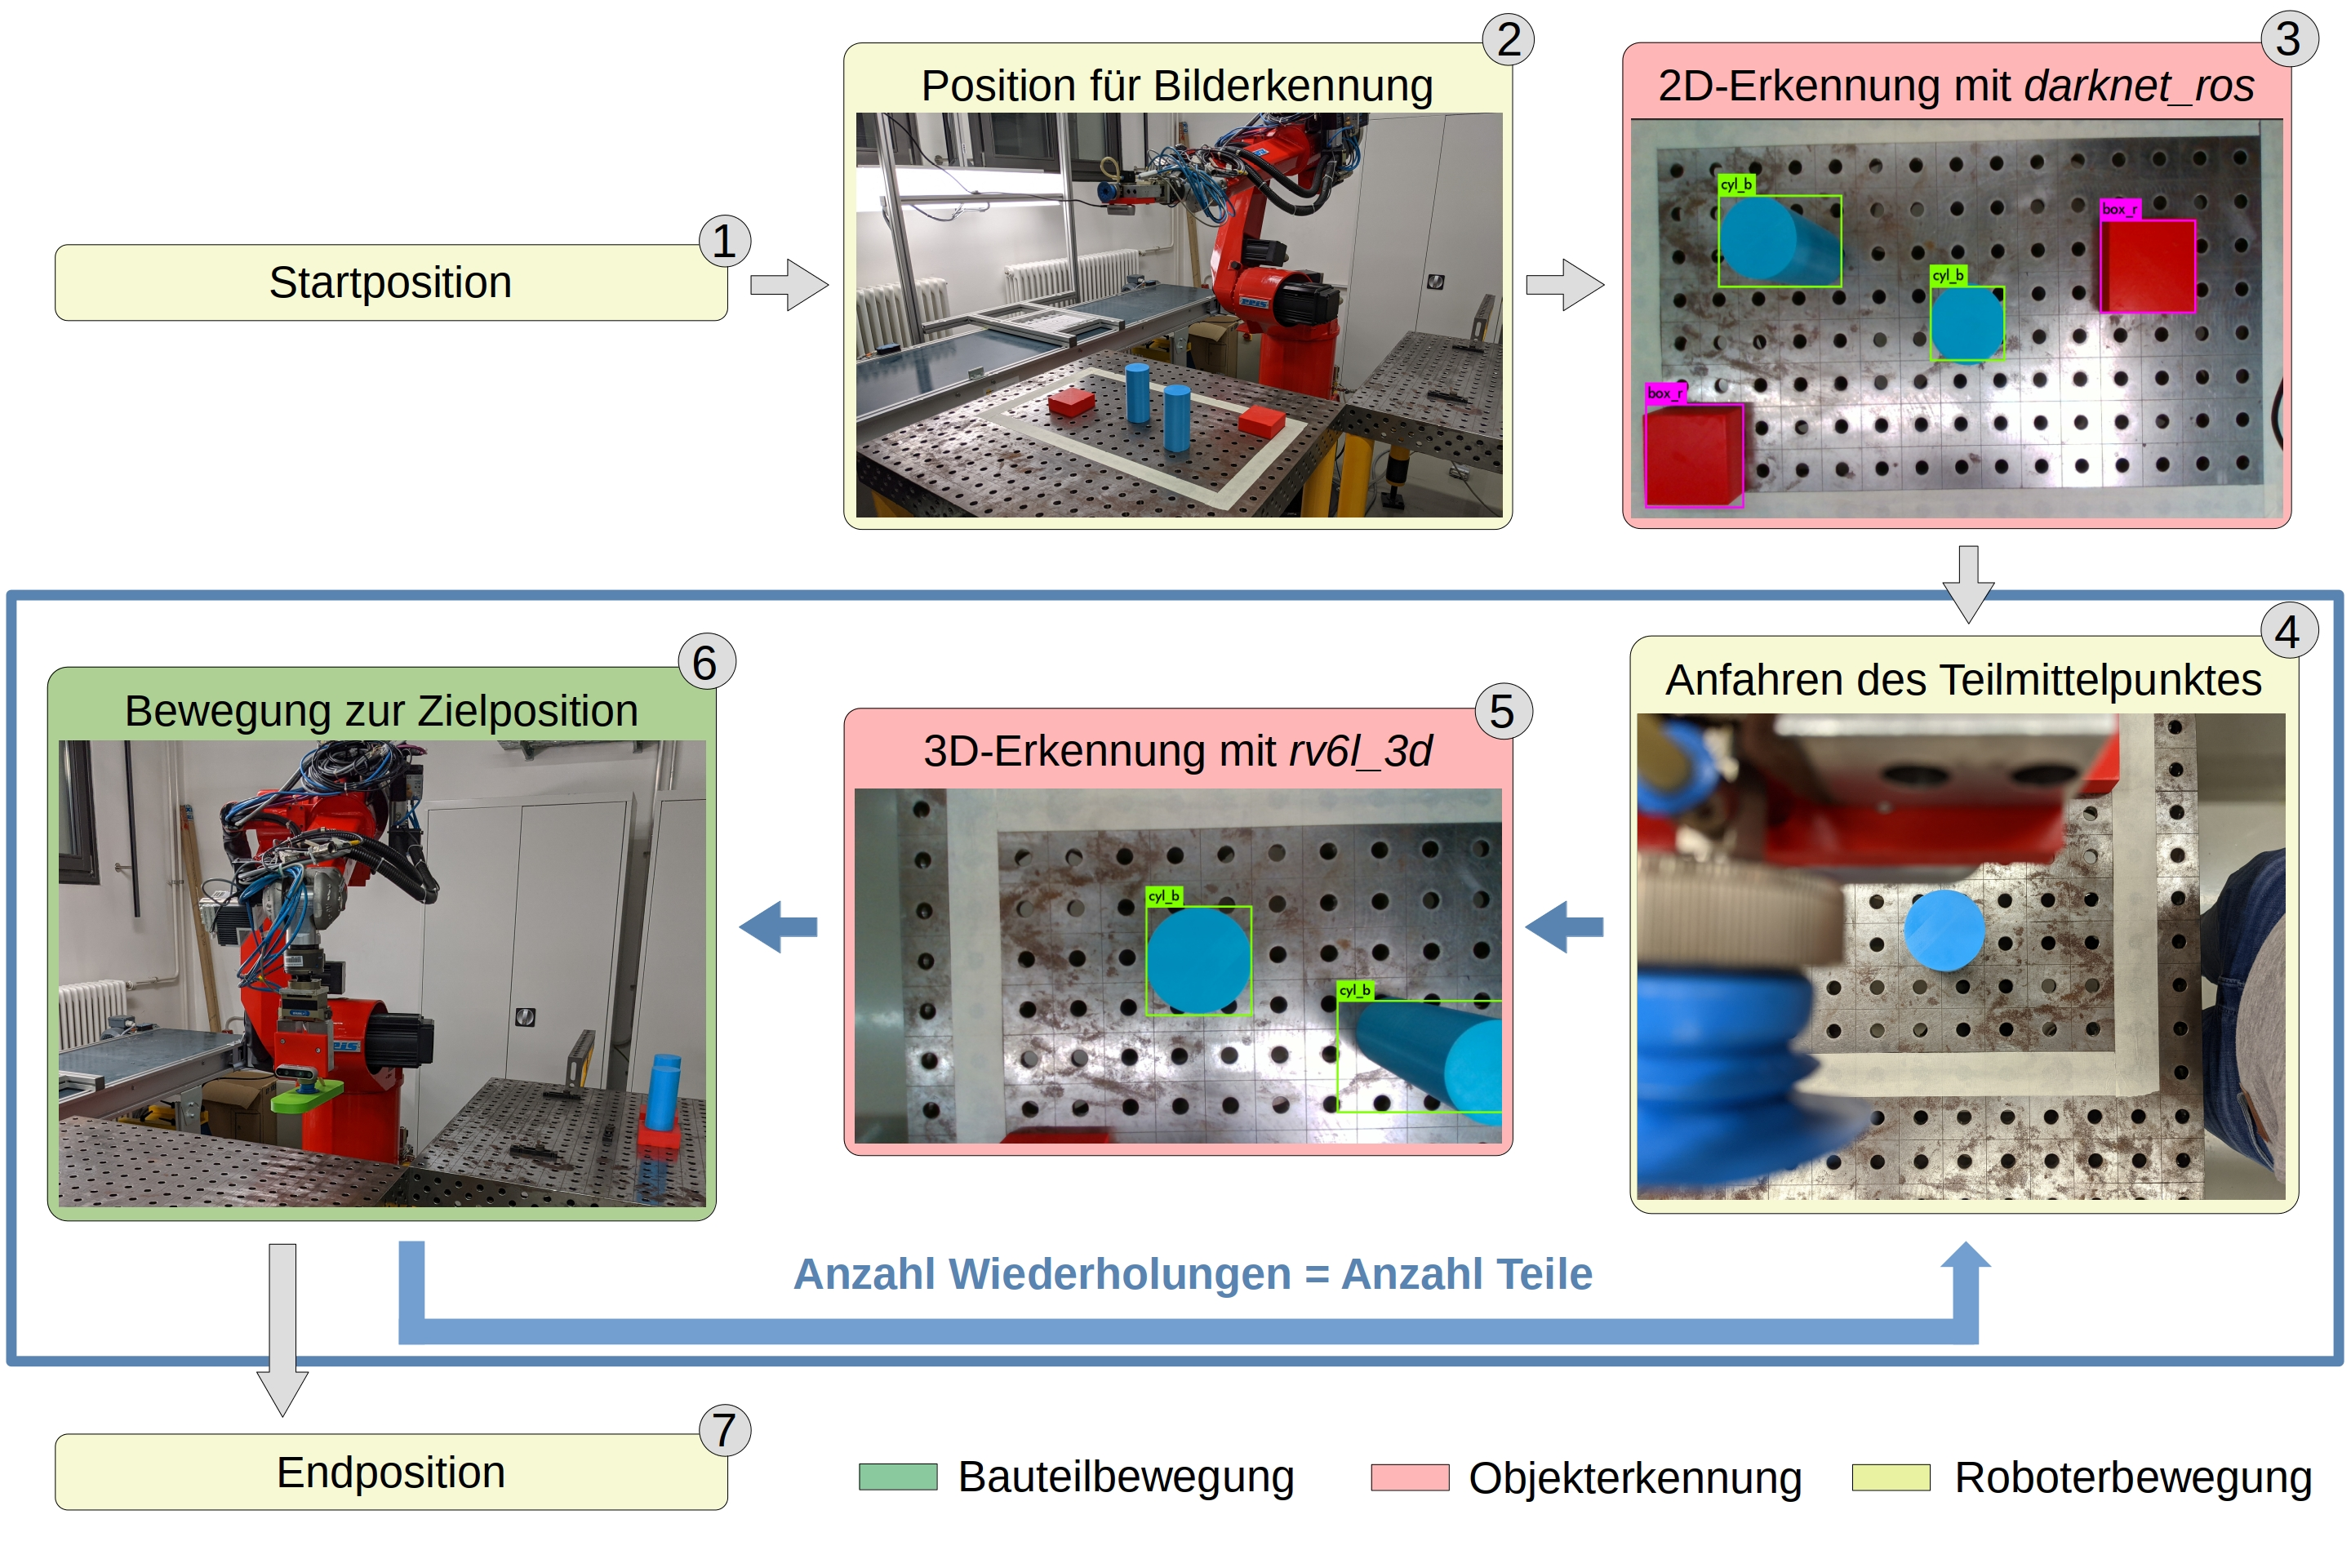
\includegraphics[angle=90, width=12cm]{Bilder/gesamtsystem_ablauf.jpg}
    \caption{Ablauf des Gesamtprogramms}
    \label{fig:gesamtsystem_ablauf}
\end{figure}